\hypertarget{jour-j-faire-le-pont-entre-loccident-et-lorient}{%
\section{Jour J : faire le pont entre l'Occident et
l'Orient}\label{jour-j-faire-le-pont-entre-loccident-et-lorient}}

\emph{Jeudi 03 mai 2018}

Ca y est ! Après les derniers préparatifs (sportifs), nous avons laissé
derrière nous notre chez-nous. Le Liban nous attend pour le début de ce
périple.

\begin{figure}
\centering
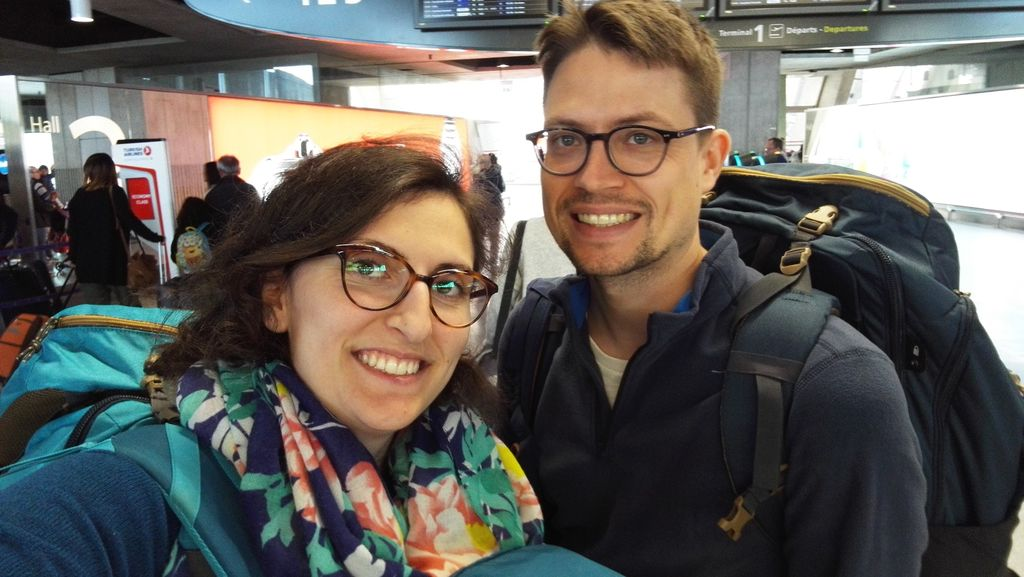
\includegraphics{images/20180503_depart.jpg}
\caption{Selfie-sac à dos de rigueur.}
\end{figure}

Est-ce qu'on réalise ce qui nous arrive ? Pas vraiment. Est-ce qu'on est
stressés ? Un peu. Une chose est sûre : on est contents :D

\begin{figure}
\centering
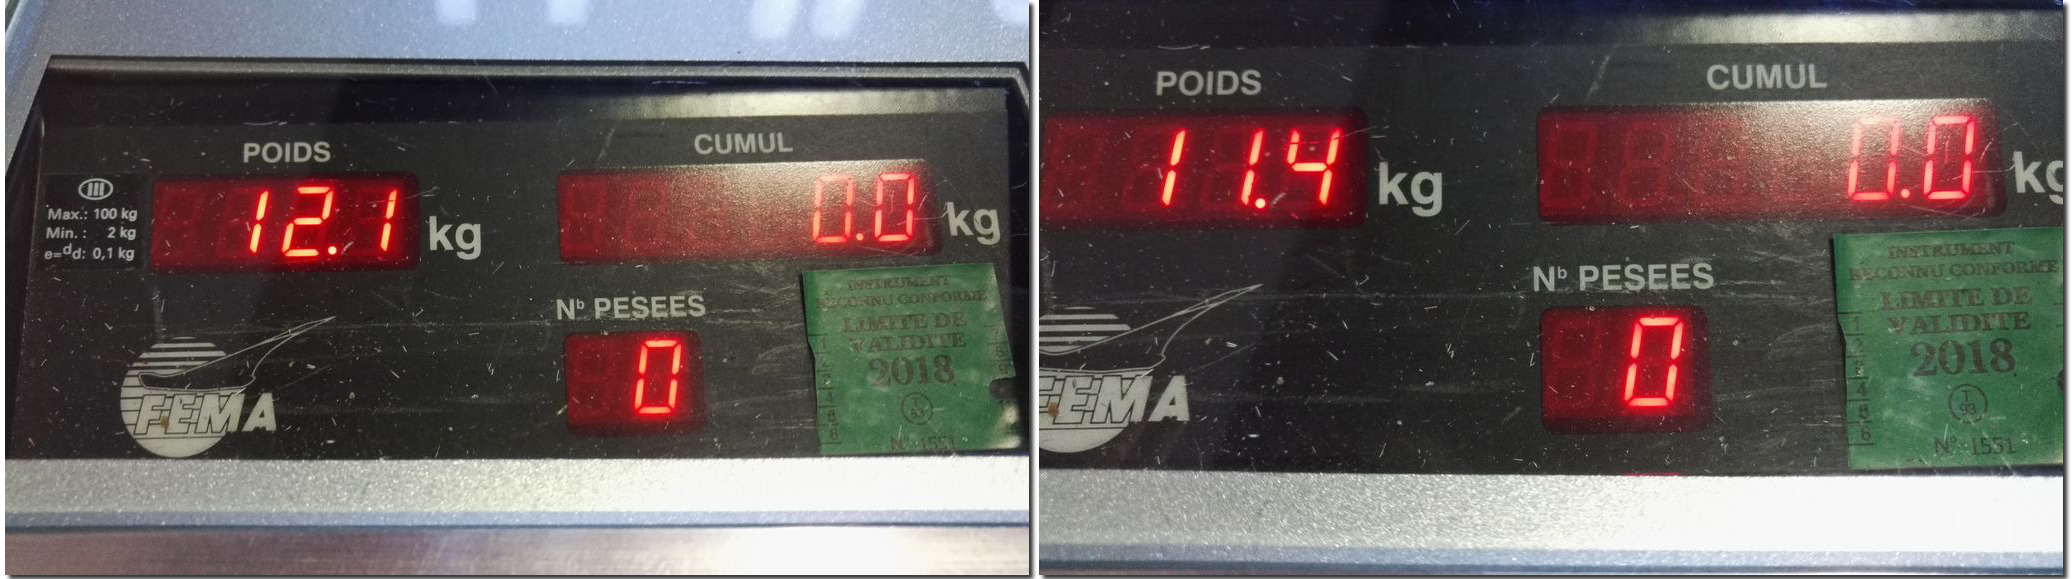
\includegraphics{images/20180503_sacs.jpg}
\caption{(gauche) Pour ceux qui n'y croyaient pas : elle l'a fait (ou presque...
aïe les 100 grammes de trop !). (droite) Florian 1 - Elida 0.}
\end{figure}

Et devinez d'où on écrit ce billet ? Istanbul, première escale d'une
longue série. On fait pas mieux comme transition entre les continents !

\begin{figure}
\centering
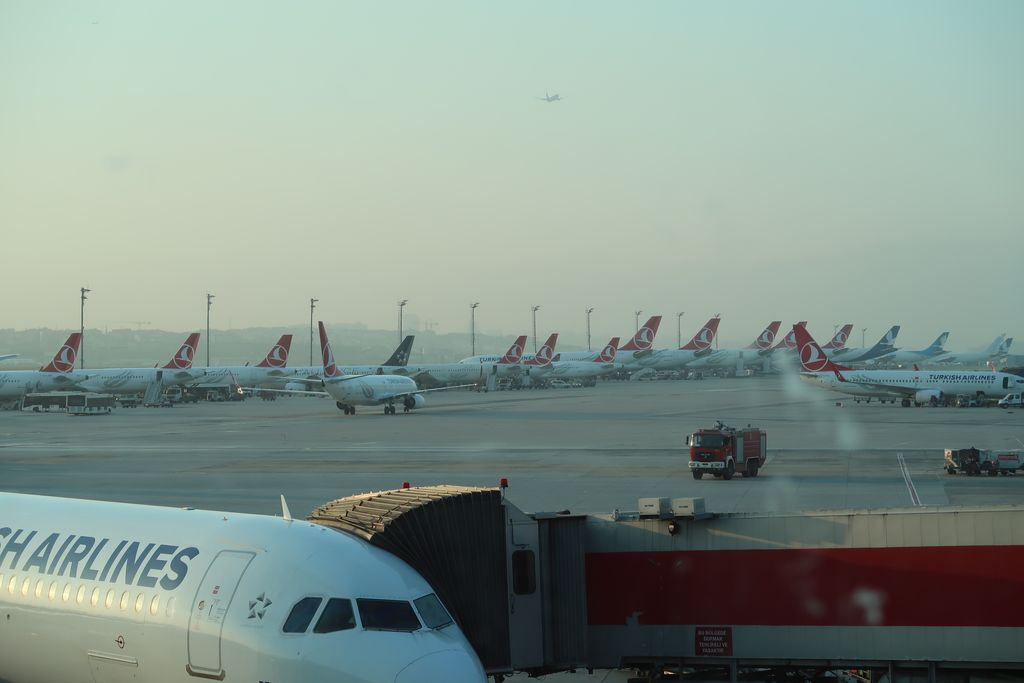
\includegraphics{images/20180503_Escale_Istanbul.JPG}
\caption{Le soleil se couche maintenant sur l'aéroport d'Istanbul (et
Flo ne rate pas une occasion de s'entraîner avec l'appareil photo ;) ).}
\end{figure}

Vite, on embarque. A très vite !

\emph{Elida et Florian}

\hypertarget{commentaires}{%
\subsection{Commentaires}\label{commentaires}}

\begin{itemize}
\item
  Thibaud, \emph{2018-05-04 12h06}

  Qu'est-ce que l'objet bleu devant Elida ? Ne serait-ce pas un gros sac
  de cabine où elle a pu caser les grammes qui manquent ? :D
\item
  Jojo, \emph{2018-05-05 11h09}

  j'espère qu'elle a donné 100g à Flo surtout ;)
\item
  Florian LB, \emph{2018-05-05 20h25}

  Oui, mais c'est elle qui porte l'ordinateur :) en vrai, on était
  surpris du fait que les gros sacs ne faisaient que 12 kilos !
\item
  Florian LB, \emph{2018-05-05 20h22}

  Thibaud, quel œil de lynx ! C'est vrai qu'on a un peu exagéré, car nos
  petits sacs pesaient bien cinq kilos supplémentaires (Elida me souffle
  qu'on emportait aussi des cadeaux... dont on va se délester à la
  première étape).
\end{itemize}
